\epigraph{\textit{The most important single aspect of sotware development is to be clear about what you are trying to build.}}{-- \textup{Bjarne Stroustrup}}

In this chapter, we will describe the first implementation of the Pregel solution, exposing the decisions that led to it, as well as the technical debt. This first version is part of Labra's publication \cite{https://doi.org/10.48550/arxiv.2110.11709}.

\section{Technology stack}

For us to describe the technologies used, we have to summarize the needs of the solution first. A large-scala data processing framework is required. What's more, a graph-processing library implementing a Pregel abstraction is also advisable; this way, we can focus on the algorithm for creating the subsets. Finally, it would be ideal if the stated technologies were open-source and well-maintained. Let us describe the chosen stack.

\begin{figure}[ht]
    \begin{subfigure}{.3\textwidth}
        \centering
        
\includegraphics[width=.7\linewidth]{img/7-1_scala.png}
        \caption{Scala programming language}
    \end{subfigure}%
    \hspace*{0.5em}
    \begin{subfigure}{.3\textwidth}
        \centering
        
\includegraphics[width=.7\linewidth]{img/7-2_spark.png}
        \caption{Apache Spark}
    \end{subfigure}%
    \hspace*{0.5em}
    \begin{subfigure}{.3\textwidth}
        \centering
        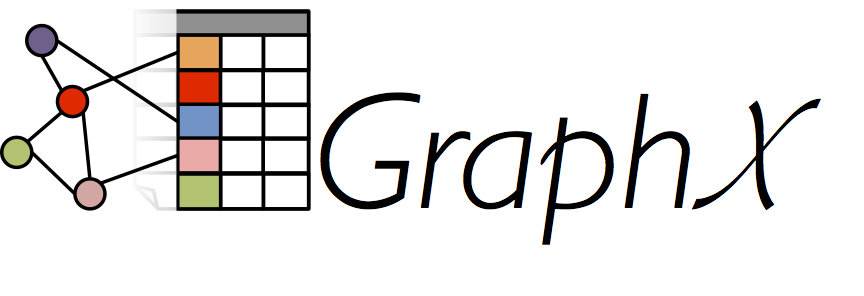
\includegraphics[width=.7\linewidth]{img/7-3_graphx.png}
        \caption{GraphX framework}
    \end{subfigure}%
    \caption{Stack of the different technologies we are using for the first solution}
\end{figure}

\subsection{Scala}

\footnotetext{\url{https://www.scala-lang.org/}}
\footnotetext{\url{https://en.wikipedia.org/wiki/Criticism_of_Java}}

Scala\footnotemark is a high-level programming language combining the object-oriented and functional paradigms. Intended to be concise and to answer the majority of Java's complaints.\footnotemark. Allowing operator overloading, a better functional support, lazy evaluation and requiring less boilerplate code. One of the features that I enjoy the most is pattern matching, which is not supported in Java. What's interesting is that Scala source code can be compiled into Java bytecode, the instruction set of the Java Virtual Machine. This way, a vast ecosystem of Java libraries are available when writing Scala programs. One of the main disadvantages of Scala is that major updates are not backwards compatible; this way, programs written in Scala 2.12 are not supported in 2.13. Not to mention that nowadays there exist two major branches of Scala development, namely Scala 2 and 3. Putting this all together, we can conclude that Scala is a bit unstable. A hell of a maintenance making loads of open-source projects and libraries get abandoned; we will discuss into this later on.

\begin{code}[Hello World written in Scala]
    \inputminted{scala}{code/listings/7-1_helloWorld.scala}
\end{code}

\subsection{Apache Spark}

Apache Spark is a Big data engine with support for several programming languages, including Scala and Python. Aiming to be simple, fast and scalable, it is the most widely-used engine in the industry. The idea behind Spark is creating a Framework that makes parallel jobs over high-volumes of data easy to write. It also bundles an engine supporting query optimization which will be discussed later on. For us to understand how Spark works, let's describe its architecture first. It follows the master-slave architecture, same idea behind the Pregel algorithm, built on top of two abstractions, namely Resilient Distributed Dataset (RDD) and Directed Acyclic Graph (DAG).

\subsubsection{RDDs (Resilient Distributed Datasets)}

We want to process graphs in parallel, hence a distributed approach is required to store the graph itself. RDDs are necessary for us to address that issue. They are spread in memory or across several machines in a cluster, and serve as Apache Spark's primary logical data unit. This method allows a single RDD to be split into numerous logical segments that can then be stored and processed on various cluster machines. RDDs are also lazy-evaluated, which saves time and boosts efficiency. For us to have a better understanding of RDDs, their main features are listed below:

\begin{itemize}
    \item \textbf{Resilience or Fault tolerance:} RDDs keep track of data lineage information to automatically restore lost data in the case of failure.
    \item \textbf{Partitioning:} Any existing RDD can be partitioned to generate mutable logical sections. This can be done by performing transformations on the current partitions.
    \item \textbf{Lazy-evaluation:} Even if you define data, it does not load in an RDD. When you call an operation, like count or collect, or when you save the output to a file system, transformations are really computed.
    \item \textbf{Immutability:} You cannot alter the data that is saved in an RDD since it is in read-only mode. But by applying modifications to the current RDDs, you can produce new RDDs.
    \item \textbf{In-memory computation:} In order to allow faster access, an RDD stores every immediately created data in main memory.
\end{itemize}

After reviewing the key aspects of RDDs, let us try to improve our understanding by describing the environment that supports this abstraction. As stated in the introduction, Spark is constructed on top of RDDs; this includes abstractions such as DataFrames and Datasets which are developed on top of them.  Every computation in Spark is carried out by RDDs under the hood. In other words, these are Spark's most basic building blocks. Some advantages of the RDDs are their simplicity, capacity to import data from heterogeneous sources, ease of caching, and the ability to apply transformations to the data stored in a functional manner. However, as we are essentially storing Java objects (or Scala ones), they consume rather large amounts of memory, garbage collection is necessary, and serialization is required for data storage and retrieval. This issue is especially critical for larger datasets since the time to serialize/deserialize grows in proportion to the amount of data stored. More into this will be discussed later on.

\subsubsection{DAG (Directed Acyclic Graph)}

The main difference between Spark and Hadoop MapReduce, whose limitations lead to the creation of the former, is the DAG Scheduler. In the context of Apache Spark, a Directed Acyclic Graph, DAG for short, is a set of Vertices, representing an RDD partition, and the Edges, representing the operations to be applied. This graph is later transformed into stages by the DAG Scheduler, where each stage contains a series of tasks to be executed in parallel. As we had seen in section \ref{section:mapReduce}, the main issue with MapReduce is having to store the result of each intermediate node, in a DAG architecture this is not required.

\begin{figure}[ht]
    \centering
    \includestandalone[width=0.65\textwidth]{diagrams/7-1_apacheSparkArchitecture}
    \caption[Architecture of Apache Spark]{Architecture of Apache Spark\footnotemark}
    \label{fig:architecture:apacheSpark}
\end{figure}

\footnotetext{\url{https://spark.apache.org/docs/0.9.1/cluster-overview.html}}

\subsection{GraphX}

A graph processing framework integrated with Apache Spark was suggested as GraphX in 2014. Its API contains a Pregel variation that is used to implement several algorithms, including PageRank. GraphX exposes an API for graphs based on RDDs~\cite{https://doi.org/10.48550/arxiv.2110.11709}.

\subsubsection{The GraphX implementation of Pregel}

GraphX provides several built-in operators for graphs\footnote{\url{https://spark.apache.org/docs/latest/graphx-programming-guide.html\#graph-operators}}. We will use the following in the rest of the paper:

\begin{itemize}
    \setlength\itemsep{1em}
    \item \mintinline[fontsize=\small]{scala}{mapVertices(g: Graph[|\VertSet|,|\EdgeSet|], f: (Id,|\VertSet|)|$\rightarrow$||\VertSet|)): Graph[|\VertSet|,|\EdgeSet|]}
          \begin{itemize}
              \item[$\blacksquare$] \textbf{Description:} Transforms each vertex attribute in the graph using the map function. It maps every pair \texttt{(id,v)} -- which are the vertices of \texttt{g} -- into \texttt{(id,f(v))}.
              \item[!] \textbf{Note:} The new graph has the same structure. As a consequence the underlying index structures can be reused.
          \end{itemize}
    \item \mintinline[fontsize=\small]{scala}{mapReduceTriplets(g: Graph[|\VertSet|,|\EdgeSet|], m: (|\VertSet|,|\EdgeSet|,|\VertSet|)|$\rightarrow$|(Id,|\MsgSet|)), r: (|\MsgSet|,|\MsgSet|)|$\rightarrow$||\MsgSet|)): RDD[Id,|\MsgSet|]}
          \begin{itemize}
              \item[$\blacksquare$] \textbf{Description:} Takes a user defined map function \texttt{m} which is applied to each triplet and can yield messages which are aggregated using the reduce function \texttt{r}.
          \end{itemize}
    \item \mintinline[fontsize=\small]{scala}{joinVertices(g: Graph[|\VertSet|,|\EdgeSet|], msgs: RDD[Id,|\MsgSet|], f: (Id,|\VertSet|,|\MsgSet|)|$\rightarrow$||\VertSet|)): Graph[|\VertSet|,|\EdgeSet|]}
          \begin{itemize}
              \item[$\blacksquare$] \textbf{Description:} Joins the vertices with the input RDD and returns a new graph with the vertex properties obtained by applying the user defined map function to the result of the joined vertices. Vertices without a matching value in the RDD retain their original value.
          \end{itemize}
\end{itemize}

The GraphX Pregel algorithm is defined iteratively where each iteration is usually called a superstep, taking as input a \texttt{Graph}[\VertSet, \EdgeSet] and the following parameters:

\begin{itemize}
    \item \texttt{initialMsg}: the message each vertex will receive at the initial iteration.
    \item \texttt{vProg}: the user-defined vertex program function which is ran on each vertex and computes a new value for it. During the first iteration, the vProg is invoked on all vertices. On subsequent iterations it is invoked only on those active vertices; that is, those receiving messages.
    \item \texttt{sendMsg}: the user-defined function that is applied to all the out edges of vertices receiving a message in the current iteration. That is, a function which computes the messages to be sent to the neighbors of a node for the next iteration.
    \item \texttt{mergeMsg}: the user-defined function that is applied to two incoming messages and merges them into one.
\end{itemize}

When this function is applied it returns the resulting graph after applying the following algorithm:

\begin{pseudocode}[Pregel algorithm as implemented in GraphX]
    \includestandalone{code/algorithms/3-1_pregel}
\end{pseudocode}

\section{Implementation of the First Pregel solution}

\section{Technical debt}

As we have exposed so far, the suggested solution is perfectly valid. The memory usage, however, is far from optimal. While we must serialize and deserialize the data at each iteration of the algorithm, making the operations to be done not efficient at all. Not to mention the lack of a query execution optimizer in RDD-based systems. There's so much room for improvement. The DataFrame's API saves the day in this regard.